\documentclass[10pt,english,aspectratio=169]{beamer}
% Use notes or hide notes or show only notes or handout


\usetheme{default}

\usepackage{xstring}
\usepackage{pgfpages}
%\makeatletter
%\IfSubStr{\@classoptionslist}{handout}
%  {\pgfpagesuselayout{2 on 1}[letterpaper,border shrink=5mm]}
%  {}
%\makeatother

\usepackage{amsmath,amssymb,amsthm}
\usepackage{stmaryrd}
\usepackage{enumerate}
\usepackage{stfloats}
\usepackage{bbm}
\usepackage{pdfpages}
\usepackage{framed}
\usepackage{tabularx}
\usepackage{scalerel}

\usepackage[most]{tcolorbox}
\tcbset{highlight math style={enhanced,
  colframe=white,colback=yellow!15,arc=8pt,boxrule=1pt,
  }}
  
\usepackage{tikz,pgf,pgfplots}
\usepackage{algorithm,algorithmic}
\usepgflibrary{shapes}
\usetikzlibrary{%
  arrows,%
  arrows.meta,
  backgrounds,
  shapes.misc,% wg. rounded rectangle
  shapes.arrows,%
  shapes,%
  calc,%
  chains,%
  matrix,%
  positioning,% wg. " of "
  scopes,%
  decorations.pathmorphing,% /pgf/decoration/random steps | erste Graphik
  shadows,%
  backgrounds,%
  fit,%
  petri,%
  quotes
}

\tikzset{background rectangle/.style={
    fill=white,
  },
  use background/.style={    
    show background rectangle
  }
}

\setbeamersize{text margin left=10mm,text margin right=35mm}

\pgfplotsset{compat=1.12}

%\usetheme{Frankfurt}
%\usecolortheme{ldpc}
\useinnertheme{rounded}
\usecolortheme{whale}
\usecolortheme{orchid}

\newcommand{\ul}[1]{\underline{#1}}
\renewcommand{\Pr}{\mathbb{P}}

%% Setup slides and notes
\makeatletter
\IfSubStr{\@classoptionslist}{notes} { \IfSubStr{\@classoptionslist}{hide} {}{\IfSubStr{\@classoptionslist}{only} {}{\setbeameroption{show notes on second screen=right}}} }{}
\makeatother
%\setbeamertemplate{note page}{\pagecolor{yellow!5}\vfill\insertnote\vfill}

\newcommand{\getpdfpages}[2]{\begingroup
  \setbeamercolor{background canvas}{bg=}
  \addtocounter{framenumber}{1}
  \includepdf[pages={#1},%
  pagecommand={%
    \expandafter\def\expandafter\insertshorttitle\expandafter{%
      \insertshorttitle\hfill\insertframenumber\,/\,\inserttotalframenumber}}%
  ]{#2}
  \endgroup}

\newcommand{\backupbegin}{
   \newcounter{finalframe}
   \setcounter{finalframe}{\value{framenumber}}
}
\newcommand{\backupend}{
   \setcounter{framenumber}{\value{finalframe}}
}

 \setbeamercolor{bibliography entry author}{fg=black}
 \setbeamercolor{bibliography entry title}{fg=black}
 \setbeamercolor{bibliography entry location}{fg=black}
 \setbeamercolor{bibliography entry note}{fg=black}
 
 \setbeamerfont{bibliography item}{size=\footnotesize}
 \setbeamerfont{bibliography entry author}{size=\footnotesize}
 \setbeamerfont{bibliography entry title}{size=\footnotesize}
 \setbeamerfont{bibliography entry location}{size=\footnotesize}
 \setbeamerfont{bibliography entry note}{size=\footnotesize}
 \setbeamertemplate{bibliography item}{\insertbiblabel}
 
\newlength\tikzwidth
\newlength\tikzheight


\newcommand{\mc}[1]{\mathcal{#1}}
\newcommand{\mbb}[1]{\mathbb{#1}}
%\newcommand{\expt}{\mbb{E}}
%\newcommand{\dd}{\mathrm{d}}
\newcommand{\Interior}[1]{\ensuremath{{#1}^{\circ}}}
\newcommand{\Closure}[1]{\ensuremath{\overline{#1}}}
\newcommand{\Complement}[1]{\ensuremath{{#1}^{c}}}

\newcommand{\Expect}{\ensuremath{\mathrm{E}}}
\newcommand{\vecnot}{\underline}
\newcommand{\RealNumbers}{\ensuremath{\mathbb{R}}}
\newcommand{\RationalNumbers}{\mathbb{Q}}
\newcommand{\ComplexNumbers}{\mathbb{C}}
\newcommand{\Real}{\mathrm{Re}}
\newcommand{\Span}{\mathrm{span}}
\newcommand{\Rank}{\mathrm{rank}}
\newcommand{\Nullity}{\mathrm{nullity}}
\newcommand{\Trace}{\mathrm{tr}}
\newcommand{\Diag}{\mathrm{diag}}
\newcommand{\dd}{\mathrm{d}}
\DeclareMathOperator*{\esssup}{ess\,sup}

% Use < , > inner product
\newcommand{\inner}[2]{{\left\langle #1 \mskip2mu , #2 \right\rangle}}
\newcommand{\tinner}[2]{{\langle #1 \mskip1mu , #2 \rangle}}

% Use < | > inner product
%\newcommand{\inner}[2]{{\left\langle #1 \mskip2mu \middle| \mskip2mu #2 \right\rangle}}
%\newcommand{\tinner}[2]{{\langle #1 \mskip1mu | \mskip1mu  #2 \rangle}}




\def\checkmark{\tikz\fill[scale=0.4](0,.35) -- (.25,0) -- (1,.7) -- (.25,.15) -- cycle;}
\def\greencheck{{\color{green}\checkmark}}
\def\scalecheck{\resizebox{\widthof{\checkmark}*\ratio{\widthof{x}}{\widthof{\normalsize x}}}{!}{\checkmark}}
\def\xmark{\tikz [x=1.4ex,y=1.4ex,line width=.2ex, red] \draw (0,0) -- (1,1) (0,1) -- (1,0);}
\def\redx{{\color{red}\xmark}}

\renewcommand{\footnotesep}{-2pt}


\begin{document}

\title{ECE 586: Vector Space Methods \\ Lecture 19: Four Fundamental Subspaces}
\author{Henry D. Pfister \\ Duke University}
\date{}
%\date{August 20th, 2020}
%\maketitle

\setbeamertemplate{navigation symbols}{}

\begin{frame}[plain]
	\titlepage
	
	\note{
		\vspace{8mm}
		\begin{enumerate}
			\setlength\itemsep{3mm}
			\color{red}
			\item Welcome to the 11th video lecture for ECE 586, Vector Space Methods. \\[2mm]
			Today, we'll finish our discussion of subspaces and bases and then move on to linear transforms.
		\end{enumerate}
	}
\end{frame}

\addtocounter{framenumber}{-1}
\setbeamertemplate{navigation symbols}{\textcolor{blue}{\footnotesize \insertframenumber ~/ \inserttotalframenumber}}




\begin{frame}{6.5: The Four Fundamental Subspaces: Basic Idea}

Consider a linear transform mapping $\mathbb{R}^n \to \mathbb{R}^m$ represented by $A\in \mathbb{R}^{m\times n}$
\vspace{1mm}

\begin{itemize}
\setlength\itemsep{2.5mm}

\item<1-> This $\vecnot{x} \mapsto A \vecnot{x}$ mapping defines \textcolor{blue}{four fundamental subspaces:} \vspace{1.5mm}
\begin{itemize}
\setlength\itemsep{1mm}
\item The \textcolor{blue}{column space} or range of $A$: $\mathcal{R}(A)$
\item The \textcolor{blue}{row space} or range of $A^T$: $\mathcal{R}(A^T)$
\item The null space: $\mathcal{N}(A)$
\item The null space of $A^T$: $\mathcal{N}(A^T)$
\end{itemize}

\vspace{0mm}

\item<2-> Notice that $\vecnot{x} \in \mathbb{R}^n$ is in the \textcolor{blue}{null space of $A$} \emph{if and only if} \vspace{-1mm}
\[ A \vecnot{x} = \begin{bmatrix} -- \text{row 1} -- \\ -- \text{row 2} -- \\ \vdots \\ -- \text{row m} -- \end{bmatrix} \begin{bmatrix}x_1 \\ x_2 \\ \vdots \\ x_n \end{bmatrix} = \begin{bmatrix} 0 \\ 0 \\ \vdots \\ 0 \end{bmatrix} \]
i.e., \textcolor{blue}{all rows of $A$ orthogonal to $\vecnot{x}$} or $\vecnot{x} \in \mathcal{R}(A^T)^\perp$
 
\item<3-> \textcolor{blue}{null space $\mathcal{N}(A)$} is the \textcolor{red}{orthogonal complement $\mathcal{R}(A^T)^\perp$ of row space}

\end{itemize}

\begin{tikzpicture}[overlay,remember picture,shift={(11.5,2.75)}]
  \node at (0,0) {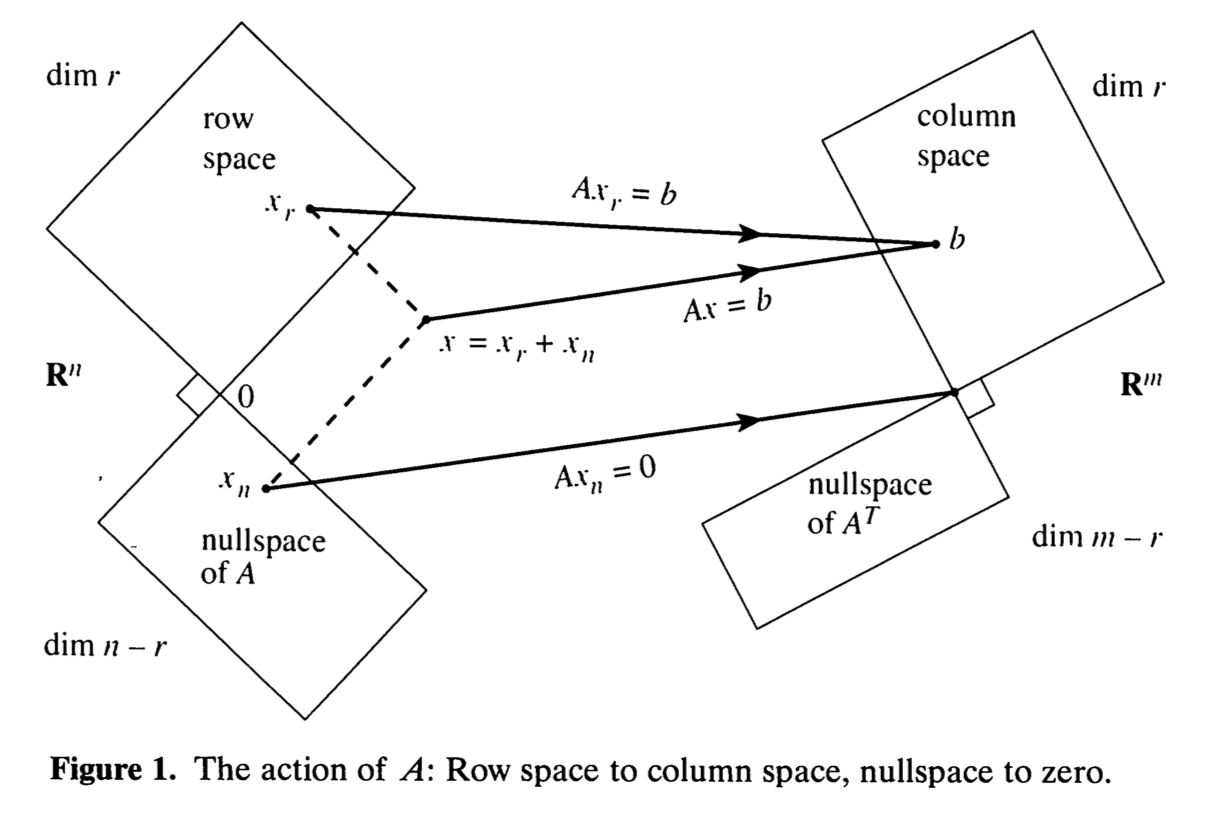
\includegraphics[width=45mm]{figures/strang_fig1.png}};
\end{tikzpicture}

\end{frame}


\begin{frame}
\frametitle{6.5: The Four Fundamental Subspaces: General Case}

\begin{itemize}
\setlength\itemsep{3mm}

\item<1-> So, \textcolor{blue}{null space of $A$} is the \textcolor{red}{orthogonal complement} of \textcolor{blue}{column space of $A^T$} 

\item<2-> Applying the same result to $A^T$ (which maps $\mathbb{R}^m \to \mathbb{R}^n$) shows \\[1.5mm] \hspace{2mm}
 \textcolor{blue}{null space of $A^T$} is the \textcolor{red}{orthogonal complement} of \textcolor{blue}{column space of $A$} 

\item<3-> This means that \textcolor{red}{$\mathcal{N}(A) = \mathcal{R}(A^T)^\perp$} and \textcolor{red}{$\mathcal{N}(A^T) = \mathcal{R}(A)^\perp$}
\end{itemize}

\begin{definition}<4-> [Adjoint]
Let $V$ and $W$ be Hilbert spaces, and assume $T \colon V \rightarrow W$ is a continuous linear transformation (i.e., $\| T \|_{\mathrm{op}} < \infty$).
Then, the \textcolor{blue}{adjoint $T^*$} is the unique linear transformation mapping $W$ to $V$ such that \vspace{-2mm}
\begin{equation*}
\inner{ T \vecnot{v} }{ \vecnot{w} }_W
= \inner{ \vecnot{v} }{ T^* \vecnot{w} }_V \quad\quad \text{for all }\vecnot{v} \in V, \vecnot{w} \in W
\end{equation*}

\vspace{-3mm}
\end{definition}

\uncover<5->{
The following 3 conditions are equivalent:
\begin{itemize}
\setlength\itemsep{1mm}
\item For all $\vecnot{w} \in W$, we have $\inner{ \vecnot{v} }{ T^* \vecnot{w} }_V = 0$
\item $\vecnot{v} \in \mathcal{R}(T^*)^\perp$
\item $\vecnot{v} \in \mathcal{N}(T)$ because $\inner{ \vecnot{v} }{ T^* \vecnot{w} }_V = \inner{ T \vecnot{v} }{ \vecnot{w} }_W = 0$ for all $\vecnot{w} \in W$
\end{itemize}
}

\end{frame}


\begin{frame}{6.5: The Four Fundamental Subspaces: Linear Equations}

\hspace*{-1mm}
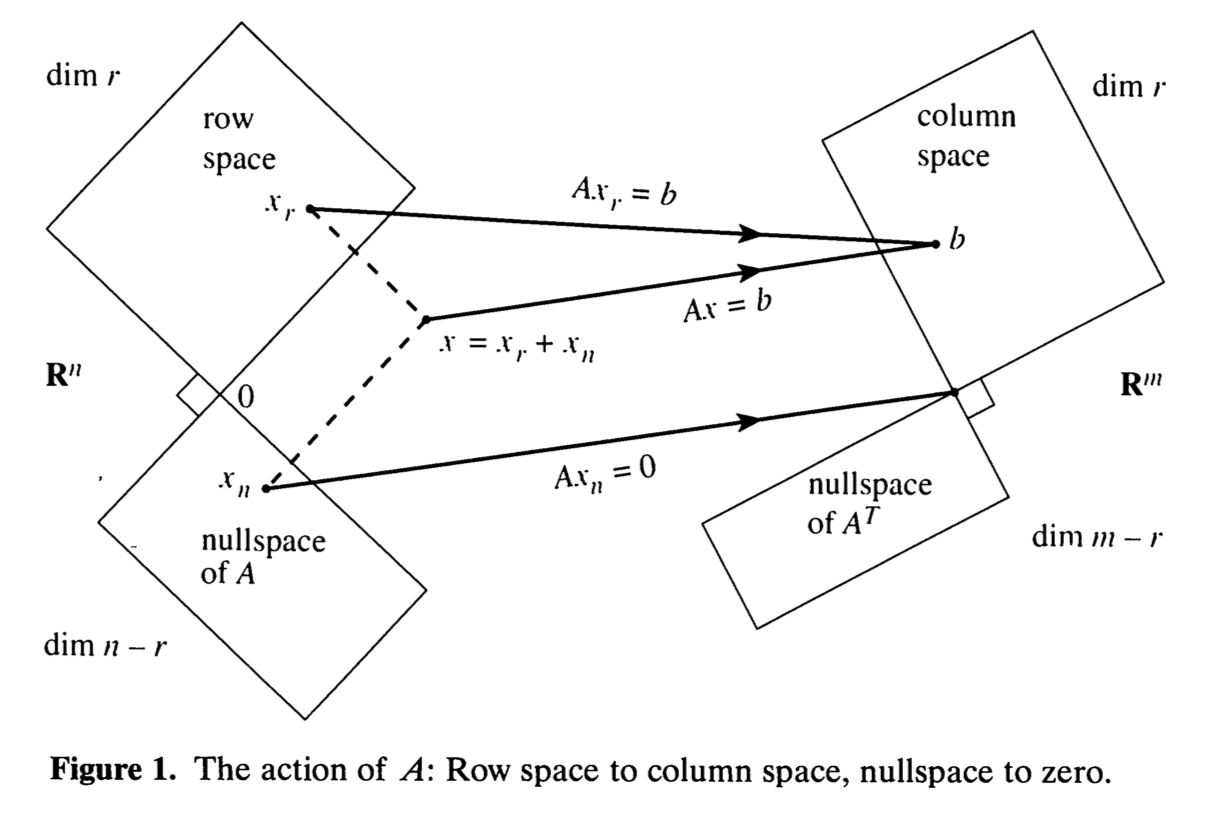
\includegraphics[width=100mm]{figures/strang_fig1.png}

\vspace{-3mm}
$r \triangleq \dim(\mathcal{R}(A))$ implies \textcolor{blue}{$\dim ( \mathcal{N}(A)) = n\!-\!r$} and \textcolor{blue}{$\dim ( \mathcal{N}(A^T)) = m\!-\!r$}

\let\thefootnote\relax\footnotetext{\hspace*{-4mm} {\tiny Figure from ``The Fundamental Theorem of Linear Algebra'' by Gilbert Strang, The American Mathematical Monthly, Nov. 1993 }}

\end{frame}

\begin{frame}{6.5: The Four Fundamental Subspaces: Least Squares}

\hspace*{-4mm}
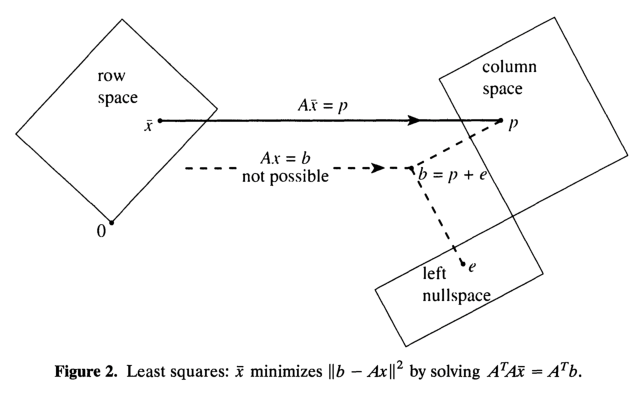
\includegraphics[width=105mm]{figures/strang_fig2}

Observe $A^T A \colon \RealNumbers^n \to \RealNumbers^n$ is invertible if non-singular (i.e., if $n=r$)

\let\thefootnote\relax\footnotetext{\hspace*{-4mm} {\tiny Figure from ``The Fundamental Theorem of Linear Algebra'' by Gilbert Strang, The American Mathematical Monthly, Nov. 1993 }}

\end{frame}

\begin{frame}{Interlude: Alternative for Linear Systems}

A ``Theorem of the Alternative'' asserts that exactly one of two logical statements is true. The following is a famous example.

\begin{theorem}
For a matrix $A \in \mathbb{R}^{m\times n}$ and a vector $\vecnot{b}\in \mathbb{R}^m$, exactly one of the following statements is true:
\begin{itemize}
\item There exists an $\vecnot{x}\in \mathbb{R}^n$ such that $A\vecnot{x} = \vecnot{b}$
\item There exists a $\vecnot{y} \in \mathbb{R}^m$ such that $A^T \vecnot{y} = \vecnot{0}$ and $\vecnot{y}^T \vecnot{b} \neq 0$.
\end{itemize} 
\end{theorem}

\begin{proof}<2->
\begin{itemize}
\item In the first case, $\vecnot{b} \in \mathcal{R}(A)$ and the four fundamental subspaces imply that $\vecnot{y}^T \vecnot{b} = 0$ (i.e., $\vecnot{y} \perp \vecnot{b}$) if $A^T \vecnot{y} = \vecnot{0}$ (i.e., $\vecnot{y}\in \mathcal{N}(A^T)$).
\item In the second case, $\vecnot{y} \in \mathcal{N}(A^T)$ implies $\vecnot{y} \perp \mathcal{R}(A)$.
So, $\vecnot{y}^T \vecnot{b} \neq 0$ implies $\vecnot{b} \notin \mathcal{R}(A)$. \qedhere
\end{itemize}
\end{proof}

%\visible<3->{Choosing $m=n$, one can also add ``for all $\vecnot{b}\in W$'' to the first statement and ``there exists $\vecnot{b}\in W$'' to the second statement.}

\end{frame}

\begin{frame} \frametitle{Next Steps}

\begin{itemize}
\setlength\itemsep{5mm}
\item To continue studying after this video -- \vspace{2mm}

\begin{itemize}
 \setlength\itemsep{3mm}
  
 \item Try the required reading from website: \\[1mm] \hspace{5mm} The Fundamental Theorem of Linear Algebra by Gilbert Strang
 
 \item Or the recommended reading:  Course Notes EF 6.5 - 6.6.1

 \item Also, look at the problems in Assignments 7 and 8
\end{itemize}
\end{itemize}

\note{
	\vspace{8mm}
	\begin{enumerate}
		\setlength\itemsep{3mm}
		\color{red}
		\item Here are some options to continue learning this material. (read) \\ [2mm]  That's it for today.  So, I'll see you next time.
	\end{enumerate}
}

\end{frame}

\end{document}


